\documentclass[UTF8,11pt,a4paper,fontset=windows]{ctexart}
\usepackage[margin=2.25cm]{geometry}
\usepackage{amsmath,amssymb,bm,booktabs,tabularx,array,graphicx}
\usepackage{caption,enumitem,float,placeins}
\usepackage[hidelinks]{hyperref}
\usepackage{fancyhdr}
\graphicspath{{assets/}}
\captionsetup{font=small,labelfont=bf}
\setlength{\parindent}{2em}
\setlength{\parskip}{0.18em}
\linespread{1.16}
\setlength{\emergencystretch}{2em}
\numberwithin{equation}{section}
\pagestyle{fancy}
\fancyhf{}
\fancyhead[L]{\small 大语言模型人类偏好数据的长度与格式关联分析}
\fancyhead[R]{\small 修订稿 v3}
\fancyfoot[C]{\thepage}
\setlength{\headheight}{15pt}
\newcolumntype{Y}{>{\raggedright\arraybackslash}X}
\newcommand{\OR}{\mathrm{OR}}
\title{\heiti 大语言模型人类偏好数据的长度与格式关联分析\\[0.3em]
\large ——基于成对比较模型与探索性路径的审计应用}
\author{程豪\quad 梁斯祯\quad 李嘉帅\quad 姜弼达\quad 翁祖成\quad 姚博晟\\
\small 中央民族大学理学院，北京 100081}
\date{}
\begin{document}
\maketitle
\thispagestyle{plain}
\begin{center}\small
基金项目：国家自然科学基金青年科学基金项目（72001197）；\\
中央民族大学创新训练项目青苗计划（QMRP2025110352）
\end{center}

\noindent\textbf{摘要：}基于LMArena的108,154条评价记录，构建成对比较模型并保留SEM探索性路径分析。明确胜负样本中，长度与粗体密度呈正关联，标题对子集敏感，列表密度证据不足。聚类推断与月份控制下主要方向保持，但长度存在明显非线性，粗体存在性未获同样支持。进一步描述明确选择状态，提出含方差估计及预算分配的分层审计方案。结果限于观察性关联，格式重解析不替代人工验证。

\noindent\textbf{关键词：}大语言模型；人类偏好；成对比较；探索性路径分析；数据审计

\begin{center}
\large\bfseries Length and Formatting Associations in Human Preference Data for Large Language Models\\[0.3em]
\normalsize An Audit Application Using Paired Comparisons and Exploratory Paths
\end{center}
\noindent\textbf{Abstract:} Using 108,154 LMArena evaluation records, this study combines a paired-comparison logistic model with exploratory observed-variable path analysis. Among decisive pairs, response length and bold density show positive conditional associations with choice. Heading associations are subset-sensitive, while list-density evidence is inconclusive. Prompt-cluster inference, model-pair clustering, month adjustment, and alternative Markdown parsing support the main density-based directions. However, restricted cubic splines reveal substantial length nonlinearity, and bold presence does not show the same association as bold density. A separate symmetric model describes whether an evaluation is decisive. The audit application retains unresolved evaluations and specifies stratified estimation, finite-population variance, and budget allocation. Path products describe candidate associations rather than causal mediation. Automated parsing agreement does not establish measurement validity; a blinded sample of 400 responses has been prepared for independent human review. The proposed audit allocation has not been validated through content review or training experiments.

\noindent\textbf{Key words:} large language models; human preference; paired comparison; exploratory path analysis; data audit

\section{引言}
大语言模型评价常采用成对比较：对同一用户问题展示两个候选回答，由用户选择较优者。该方式能够直接记录实际使用中的相对偏好，Chatbot Arena 等平台据此开展众包评价与模型比较\cite{chiang}。然而，一个回答被选中并不等于其所有可观察特征都具有同样的质量含义。较长回答可能提供更多必要信息，也可能包含重复解释；标题、列表和粗体可能改善信息组织，也可能仅改变文本外观。对评价数据使用者而言，需要判断选择结果与这些形式特征之间存在多大关联，从而决定哪些配对应进入进一步复核。

已有研究从不同角度讨论偏好信号的构成。Li 等\cite{li}通过细粒度属性分析比较人类与大语言模型的偏好，表明总体选择背后包含多种评价维度。Dubois 等\cite{dubois}利用回归控制长度因素，改进自动评价指标对长度差异的处理。Zhang 等\cite{zhang}进一步考察列表、粗体等格式模式，说明格式与偏好学习之间的关系值得独立研究。这些工作为偏好数据审计提供了依据，但人类评价与自动评价器输出是不同的研究对象，对自动评价器的校正效果不能直接转化为人类选择中的因果结论。

在真实成对数据中，长度与格式分析还面临两个相互联系的问题。其一，格式计数随文本扩展而变化，仅比较胜者与败者的格式总量，难以判断关联来自格式本身还是文本规模。其二，不同模型的输出习惯、任务分布和被选择概率可能同时不同，忽略模型身份会使形式指标吸收模型间差异。因此，实际分析既要保持成对比较单位的一致性，也要在同一回归中联合纳入长度、格式和可观测背景信息。

本文以 LMArena 公开人类偏好数据为对象，研究三个问题：明确胜负配对的长度与格式差异如何分布；联合调整可观测变量后，哪些关联仍有统计支持；这些结果如何转化为可操作的审计分层。方法上，将长度对数比、格式密度差与模型身份对比项放入同一 Logistic 模型，并结合配对检验和敏感性分析评估结果。同时保留 SEM 框架下的观测变量探索性路径分析，描述长度、格式与选择的候选关联结构。应用上，使用真实样本构建长度分层报告，给出固定复核预算下的抽样方案。本文的贡献在于将配对建模与评价数据复核衔接起来，并明确不同格式指标的证据差异。研究目标限定为观察性关联及其审计用途，形式编辑的因果效果需由独立干预设计检验。

\section{数据与指标构造}
\subsection{数据来源与样本边界}
研究使用 \texttt{lmarena-ai/arena-human-preference-140k} 的本地冻结数据\cite{dataset}，共 7 个原始分片、135,634 条记录。数据同时包含会话标识、评价次序、双方对话、胜负标签及长度和格式元数据。本文按会话首轮评价建立比较单位，检查角色交替、两侧用户输入轨迹一致性、文本有效性、标签完整性及计数合法性。通过筛选后，对仍存在多条候选记录的会话整体排除，得到每个唯一会话一条记录的分析集。

按首次失败原因互斥计数，排除非首轮评价 27,319 条、语言异常 30 条、空或无效文本内容 109 条、会话记录歧义 22 条，最终保留 108,154 条。评价结果包括 A 胜 39,042 条、B 胜 39,917 条、平局 16,574 条、双方差 12,621 条。后两类保留用于描述、明确选择状态建模和审计分层，不并入条件胜负模型；因此，回归样本为 78,959 对明确胜负记录。其分析目标是该筛选总体中的相对选择，而不是所有平台交互中的偏好。

首轮评价与单轮对话需要区分：首轮评价记录内部仍可能包含多轮用户与模型交互，长度和格式由该评价记录的汇总字段表示。限制为首轮有助于减少评价历史与当前测量混杂，但不保证全部计量误差被消除。不同会话仍可能来自同一用户或相同提示词，故会话唯一性不能直接作为观测相互独立的证据。

\subsection{结果变量与形式指标}
对第 $i$ 个明确胜负配对，令 $Y_i=1$ 表示 A 侧胜出，$Y_i=0$ 表示 B 侧胜出。记双方回答 token 总量为 $L_{Ai}$、$L_{Bi}$，二者均为正数。长度指标定义为
\begin{equation}
 x_{Li}=\log\frac{L_{Ai}}{L_{Bi}}.
\end{equation}
与绝对差相比，对数比描述相对长度差异，并在交换双方后改变符号。例如，200 对 100 tokens 与 2,000 对 1,000 tokens 对应相同的长度比。该度量不把相同的绝对差视为相同的相对扩展，也不能替代任务所需信息量的测量。

记格式类型 $f\in\{H,B,S\}$ 分别代表标题、粗体和列表，双方格式计数为 $C_{fAi}$、$C_{fBi}$。定义每千 token 密度差
\begin{equation}
 x_{fi}=1000\left(\frac{C_{fAi}}{L_{Ai}}-\frac{C_{fBi}}{L_{Bi}}\right).
\end{equation}
格式计数沿用上游元数据：标题为 h1--h6 计数之和，列表为有序与无序列表计数之和，粗体为两种标记计数之和。主分析使用上游计数；补充分析使用Mistune AST重新解析全部助手消息，按标题块、列表条目和strong片段分别计数，排除代码和原始HTML节点，并逐消息累加。重解析只构成替代测量，不是人工金标准；两种口径均不等于结构质量或视觉效果。密度可以减少文本规模对格式总量的直接影响，但仍共享长度分母，不能据此认为长度与格式已完全分离。

描述检验使用胜者减败者的差值；回归始终保持原始 A/B 方向，不按照胜负重新排列解释变量。主模型将四个形式指标统一按全量明确胜负样本标准化，即 $z_{ki}=(x_{ki}-\bar x_k)/s_k$，其中 $s_k$ 采用分母为78,959的标准差；英语、单轮和密度敏感性模型均沿用该尺度。

\begin{table}[htbp]\centering\small
\caption{主要变量及统计含义}\label{tab:vars}
\begin{tabularx}{\textwidth}{p{2.8cm}Y Y}
\toprule
变量 & 定义与来源 & 解释边界\\
\midrule
胜负 $Y_i$ & A 胜为 1，B 胜为 0 & 排除平局与双方差后的条件总体\\
长度 $x_{Li}$ & 双方 token 总量的对数比 & 相对文本规模，不代表信息增益\\
格式 $x_{fi}$ & 标题、粗体、列表每千 token 密度差 & 依赖上游计数，共享长度分母\\
任务及提示词 & 任务标签、七类提示词属性、输入长度、轮数及语言 & 不是逐条回答内容质量评分\\
模型身份 & A、B 两侧模型指示变量之差 & 控制模型间平均差异，不等于题目级质量控制\\
\bottomrule
\end{tabularx}
\end{table}

\subsection{控制变量与敏感性子集}
任务信息包括创意写作、指令遵循、数学和代码标签。七类提示词属性对应复杂性、创造性、领域知识、问题求解、现实情境、具体性和技术准确性需求，其取值来自任务标注，不能解释为回答已达到相应质量标准。另纳入用户输入 token 数的 $\log(1+L_U)$、对话轮数和语言虚拟变量；各分析子集中频数低于 100 的语言合并为低频类别。

模型身份采用双方模型指示变量的差表示，不使用由本批胜负标签估计的模型胜率作为解释变量。为检查语言混合及对话轮次口径的影响，另对英语样本 42,001 对和单轮对话样本 67,608 对拟合相同类型模型。二者与全量样本重叠，属于敏感性检查；本次统一标准化单位，但重叠子集的点估计差异仍不构成独立复制或正式异质性检验。


按唯一记录id从原始分片连接时间及用户文本，全部108,154条记录匹配且时间无缺失，覆盖2025年4月17日至7月24日的4个自然月。原始schema没有稳定用户标识，不能把唯一会话视为唯一用户。

\section{成对比较模型与推断方法}
\subsection{描述性配对比较}
以胜者减败者的差值描述方向，报告非零差配对中正差比例、零差数及秩二列相关。符号检验及格式存在性的精确McNemar检验沿用冻结分析；全量、英语、单轮及任务组合的比较采用同一Holm家族校正\cite{holm}。这些描述检验以配对独立为工作假设，仅作背景，不替代下文的聚类回归推断。补充Wilcoxon结果不作无条件的中位数检验解释。

\subsection{含模型身份对比项的Logistic模型}
对明确胜负样本，令$p_i=\Pr(Y_i=1\mid\bm z_i,\bm X_i,m_{Ai},m_{Bi})$，拟合
\begin{equation}\label{eq:logit}
 \log\frac{p_i}{1-p_i}=\alpha+\beta_Lz_{Li}+\beta_Hz_{Hi}
 +\beta_Bz_{Bi}+\beta_Sz_{Si}+\bm\gamma^\top\bm X_i
 +\theta_{m_{Ai}}-\theta_{m_{Bi}}.
\end{equation}
模型身份参数差沿用Bradley--Terry型结构\cite{bradley,firth}，通过指定参考模型识别。本文称其为含模型身份对比项的成对比较Logistic模型，区别于匹配病例的条件Logistic回归。共有任务变量及截距允许A侧优势随背景变化，不将模型宣称为严格交换对称的纯排名模型。参数通过最大化Bernoulli对数似然估计：
\begin{equation}
 \ell(\bm\eta)=\sum_i\{Y_i\bm v_i^\top\bm\eta-\log[1+\exp(\bm v_i^\top\bm\eta)]\}.
\end{equation}
检查比较图连通性、设计矩阵秩、收敛与参数有限性，并以替换参考模型核验焦点系数和预测概率不变。连通和收敛不等于模型设定正确；数值诊断也不替代完全分离的形式化证明。

\subsection{聚类协方差与多重比较}
提示词分组先统一Unicode NFC及换行符，再对消息序列计算哈希；保留空格和代码缩进，不作语义近似去重。主要推断按首条用户消息聚类，完整用户消息序列及无序模型对聚类作为另外两种敏感性方案。三种聚类分别计算，未进行多向聚类；它们均不能替代缺失的用户标识。

设组$g$的得分和为$\bm s_g=\sum_{i\in g}\bm v_i(Y_i-\widehat p_i)$，$B=\sum_i\widehat p_i(1-\widehat p_i)\bm v_i\bm v_i^\top$，聚类协方差为\cite{cameron}
\begin{equation}
 \widehat V_{\mathrm{cl}}=\frac{G}{G-1}\frac{n-1}{n-K}
 B^{-1}\left(\sum_{g=1}^G\bm s_g\bm s_g^\top\right)B^{-1},
\end{equation}
其中$G$为簇数，$K$为参数数目。系数区间和双侧检验采用$t_{G-1}$近似；HC0使用正态近似作为对照。组内可相关而组间独立仍是工作假设。簇规模不均衡及模型对间共享同一模型的相关性可能影响近似，不能将任一方案视为全面消除依赖。

主分析在全量、英语、单轮三个模型的12个焦点系数间实施Holm校正，各协方差方案分别构成一族。月份、替代解析、格式存在性和截尾四种补充模型的16个系数构成另一族；明确胜负状态模型的4项构成独立家族。95\%区间均为逐项区间。优势比$\exp(\beta_k)$对应全量明确胜负样本一个标准差，不能解释为编辑文本后的因果收益。格式存在性模型另用该二元差值的全量标准差，不能与密度OR直接比较。

\subsection{非线性及其他敏感性设定}
长度项使用四节点限制性三次样条\cite{harrell}，节点规则在拟合前固定为全量长度指标的5\%、35\%、65\%、95\%分位数；保留线性项并增加两个非线性基函数。对两个非线性系数联合检验，聚类方案采用$F_{2,G-1}$近似。AIC只作为条件独立似然下的辅助描述。

预测曲线将有方向长度比$r=L_A/L_B$固定在给定值，对观察样本其余协变量分布平均：
\begin{equation}
 \widehat P(r)=\frac1n\sum_i\operatorname{logit}^{-1}
 \{\widehat\eta_i+\widehat f(z_L(r))-\widehat f(z_{Li})\}.
\end{equation}
区间采用首提示词聚类协方差与Delta法，为逐点区间。曲线保留格式密度不变，只表示模型标准化预测关联；固定密度而改变长度隐含计数变化，不能理解为保持回答其余内容不变的长度干预。

其他检查分别加入月份固定效应、用AST重解析计数替换上游格式计数、改用格式有无差，以及排除长度对数比两端各1\%的配对。替代计数使用原密度尺度以便解释，存在性模型单独标准化。敏感性设定一次改变一个方面，没有依据显著性筛选变量。月份主效应不代表控制了所有模型随时间变化的异质性。

\subsection{明确胜负与未决状态}
令$D_i=1$表示明确胜负，平局和双方差对应$D_i=0$。全部保留记录上拟合
\begin{equation}
 \operatorname{logit}\Pr(D_i=1)=\alpha_D+\delta_Lw_{Li}
 +\sum_f\delta_fw_{fi}+\bm\gamma_D^\top\bm X_i
 +\phi_{m_{Ai}}+\phi_{m_{Bi}}+\lambda_{t_i},
\end{equation}
其中$w$为长度对数比及格式密度差绝对值在全部保留样本中的标准化量，$\lambda_{t_i}$为月份项；模型身份以加和而非差分编码，使方程在A/B交换后不变。此方程描述是否形成明确选择，与条件胜负模型共同区分两个研究对象。虽然$\Pr(\text{A胜})=\Pr(D=1)\Pr(\text{A胜}\mid D=1)$，增加状态方程并不能自动纠正未观测混杂或样本选择偏差。平局和双方差仍分别报告，不把二者解释为同一种评价。

\subsection{审计分层}
定义无方向长度比
\begin{equation}\label{eq:ratio}
 R_i=\frac{\max(L_{Ai},L_{Bi})}{\min(L_{Ai},L_{Bi})},
\end{equation}
按$R\leq1.25$、$1.25<R\leq2$、$R>2$形成三个复核层，并保留各层全部评价状态。阈值为事后解释性规则，未证明最优；关联强弱只提示复核方向，不判定标签错误。第6节区分层间比较与总体争议率估计，给出相应预算分配。
\section{实证结果与敏感性分析}
\subsection{描述结果及主模型}
明确胜负样本中有187对等长，78,772对不等长；较长回答获胜49,130对，占62.37\%。胜者减败者的中位长度差为125 tokens。标题、粗体、列表密度较高者的未调整获胜比例分别为55.30\%、55.80\%、50.33\%，各自非零差分母为49,087、70,187和69,296。这些描述比例不衡量独立格式作用。

全量比较图包含52个模型，形成一个连通分量；主设计矩阵秩为90，英语和单轮分别为69和89。拟合收敛，未出现分离警告，更换参考模型后焦点系数和预测概率保持数值一致；尚未完成线性规划式分离检验。首提示词有75,862簇，其中73,826为单例，最大簇10条；完整序列有76,213簇；无序模型对有1,201簇，最大簇267条。提示词重复较少解释了其标准误与HC0接近，但不能据此排除同用户跨提示词的依赖。

表\ref{tab:reg}采用首提示词聚类推断。全量长度OR为1.6196；其单位为长度对数比增加全量标准差1.0224，相当于原长度比乘以约2.780，不是增加一个token。该OR是线性设定的平均斜率摘要，后文的非线性检验表明不能将其视为所有长度区间共同适用的恒定关联。

\begin{table}[htbp]\centering\small\caption{统一标准化下的条件选择关联}\label{tab:reg}
\begin{tabular}{llrrr}\toprule
样本 & 特征 & OR & 95\%区间 & Holm $p$\\\midrule
全量 & 长度对数比 & 1.6196 & [1.5798, 1.6603] & $<0.001$\\
全量 & 标题密度差 & 1.0282 & [1.0091, 1.0477] & 0.0218\\
全量 & 粗体密度差 & 1.0556 & [1.0339, 1.0778] & $<0.001$\\
全量 & 列表密度差 & 0.9872 & [0.9703, 1.0043] & 0.5652\\
英语 & 长度对数比 & 1.5866 & [1.5336, 1.6415] & $<0.001$\\
英语 & 标题密度差 & 1.0107 & [0.9885, 1.0335] & 0.7162\\
英语 & 粗体密度差 & 1.0701 & [1.0438, 1.0971] & $<0.001$\\
英语 & 列表密度差 & 0.9894 & [0.9695, 1.0098] & 0.7162\\
单轮 & 长度对数比 & 1.6303 & [1.5876, 1.6742] & $<0.001$\\
单轮 & 标题密度差 & 1.0211 & [1.0010, 1.0417] & 0.1987\\
单轮 & 粗体密度差 & 1.0574 & [1.0343, 1.0811] & $<0.001$\\
单轮 & 列表密度差 & 0.9890 & [0.9710, 1.0074] & 0.7162\\\bottomrule\end{tabular}
\par\smallskip\footnotesize 注：全量78,959对，英语42,001对，单轮67,608对；首提示词聚类。12项为一个校正家族。
\end{table}

全量标题关联较弱，英语子集区间跨1，单轮标题虽逐项区间略高于1，Holm校正后仍不显著；粗体密度在三个样本中保持正关联，列表密度均缺乏明确支持。模型身份项只能吸收平均模型差异，不能测量具体回答的正确性或必要信息量。
\begin{figure}[htbp]\centering
\includegraphics[width=\textwidth]{adjusted_associations.pdf}
\caption{三个重叠样本的条件关联。统一标准化尺度，首提示词聚类逐项区间；左右面板横轴范围不同。}\label{fig:reg}\end{figure}

\subsection{聚类 时间及函数形式}
将首提示词聚类改为完整序列或模型对聚类后，全量标题仍通过各自方案的Holm校正；模型对方案的标题校正$p=0.0275$，粗体为$p<0.001$。因此本次结果不支持“聚类必然使标题消失”的预设判断，但标题的子集敏感性仍然存在。
月份调整后的长度OR为1.6195，粗体密度为1.0556；去除长度比两端各1\%后长度OR升至1.7630，说明总体线性斜率对尾部范围敏感。限制性三次样条的非线性联合检验在首提示词聚类下$p<0.001$，模型对聚类下亦$p<0.001$。原始对数比节点约为$-1.6409,-0.3448,0.3442,1.6551$，对应长度比约为0.194、0.708、1.411、5.234。
\begin{figure}[htbp]\centering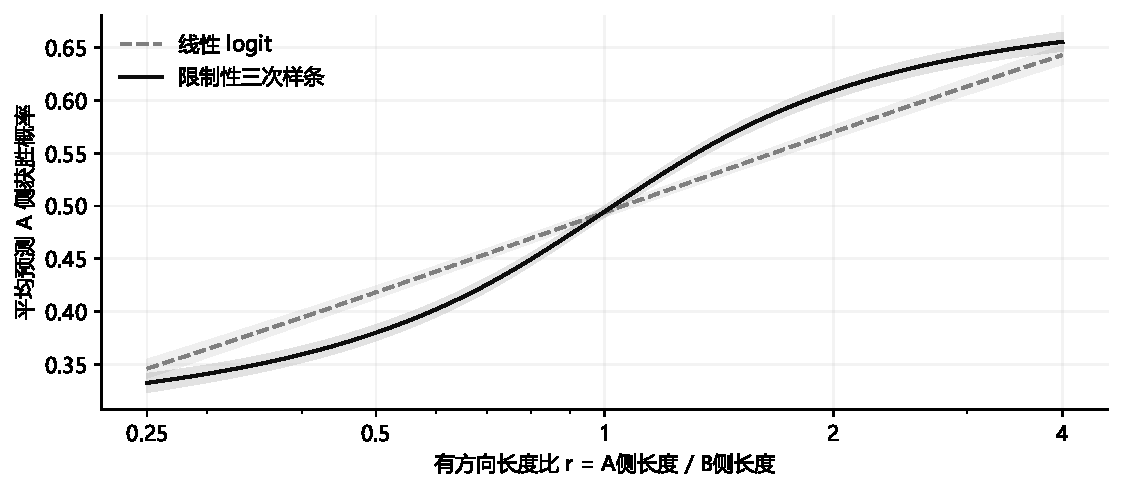
\includegraphics[width=.94\textwidth]{length_curve.pdf}
\caption{长度与选择的标准化预测关联。阴影为首提示词聚类Delta法95\%逐点区间，固定观察到的格式密度与其他协变量，横轴为A/B有方向长度比。}\label{fig:curve}\end{figure}

图\ref{fig:curve}显示线性与样条在不同长度范围的拟合差异。曲线展示0.25至4的长度比，该区间位于观察长度比的1\%至99\%分位范围内；但边际范围内不保证全部协变量组合都有共同支持。非线性显著不自动确定最优复核阈值，也不证明某一长度比例是因果拐点。

样条结果方程下，标题、粗体及列表密度OR分别为1.0297、1.0564、0.9924，三个格式项的Holm校正值依次为0.0045、$<0.001$、0.3855。完整敏感性表同时保留原线性基准，避免只报告符合预期的设定。

\subsection{明确选择状态与格式测量}
平局和双方差合计29,195条，占保留样本约26.99\%。表\ref{tab:decisive}考察是否产生明确胜负，单位为全部保留样本中绝对差指标的一个标准差。它与表\ref{tab:reg}使用不同结果变量和尺度，不能横向比较OR大小或把状态模型称为选择偏差校正。

\begin{table}[htbp]\centering\small\caption{形成明确胜负的关联}\label{tab:decisive}
\begin{tabular}{lrrr}\toprule
特征 & OR & 95\%区间 & Holm $p$\\\midrule
长度对数比绝对值 & 1.2137 & [1.1923, 1.2354] & $<0.001$\\
标题密度差绝对值 & 1.0357 & [1.0200, 1.0517] & $<0.001$\\
粗体密度差绝对值 & 0.9970 & [0.9814, 1.0127] & 0.7045\\
列表密度差绝对值 & 1.0526 & [1.0355, 1.0700] & $<0.001$\\\bottomrule\end{tabular}
\par\smallskip\footnotesize 注：108,154条，控制月份及对称模型身份项，首提示词聚类；4项校正。
\end{table}

长度差异、标题及列表密度差异与形成明确选择正相关，粗体密度绝对差缺乏同样证据。这表明“是否明确选择”与“明确选择后哪侧获胜”应分开讨论。

对216,308个侧别回答，AST重解析与上游计数的完全一致率，标题为98.96\%、列表97.89\%、粗体96.88\%；存在性一致率分别为99.55\%、99.68\%、99.85\%。这些是口径一致性，不是相对于人工真值的准确率。替代计数模型中，长度OR为1.6187、粗体密度OR为1.0569，主要方向与原计数接近。

然而，改用格式存在性后，粗体差值OR为1.0088，95\%区间[0.9869, 1.0312]，校正$p=0.8660$，未获得明确关联证据。因而结论应限定为粗体密度，不能泛化成“使用粗体即可提高被选择概率”。存在性与密度的单位和研究问题不同。

已按上游三种格式存在性组合分8层，每层随机抽取50个回答，共400个，隐藏模型、胜负与自动计数，准备独立双人复核和裁决。因尚未取得人工标注，本稿不报告人工precision、recall或内容质量改善。稀有语法边界另由可复现代码样例检查，不冒充概率样本的人工验证。

\FloatBarrier
\section{探索性路径分析}
\subsection{观测变量广义路径框架}
保留SEM框架下的探索性尝试，以长度指向标题、列表、粗体密度，再由格式指向选择，同时保留长度至选择的路径。这里没有潜变量或测量模型；三个连续格式方程采用OLS，二元选择方程采用Logistic，并允许格式残差相关。对$k\in\{H,S,B\}$，有
\begin{equation}
 z_{ki}=\alpha_k+a_kz_{Li}+\bm\gamma_k^\top\bm X_i
 +\theta_{k,m_{Ai}}-\theta_{k,m_{Bi}}+\varepsilon_{ki}.
\end{equation}
选择方程使用式\eqref{eq:logit}，格式系数记为$b_k$。方向为事后探索设定，无时间先后或干预识别；不使用由同一样本胜率构造的能力代理，也不因列表不显著而删除其路径。

对七个焦点系数，先计算同一配对对各方程估计的影响贡献，再按首提示词求和形成跨方程聚类夹心协方差；完整序列和模型对方案作敏感性分析。方程间使用各自参数数目进行有限样本修正，保留$a$与$b$的估计相关。三个子集共21条路径在每种协方差方案内实施Holm校正。

从联合渐近正态分布模拟50,000次参数，种子20260921，取$a_kb_k$的2.5\%及97.5\%分位数。该区间条件于观察到的标准化尺度，为逐项参数模拟区间，不是Bootstrap，也未经多重校正。$a_kb_k$只用于描述线性工作模型中的候选关联通路，不是概率变化、自然间接效应或中介比例；不将其与长度系数相加解释为约简Logistic模型的总效应。
\subsection{路径结果与模型依赖}

\begin{table}[htbp]\centering\small\caption{探索性路径乘积}\label{tab:paths}
\begin{tabular}{llrr}\toprule
样本 & 候选通路 & 乘积 & 95\%模拟区间\\\midrule
全量 & 长度$\to$标题$\to$选择 & 0.00429 & [0.00141, 0.00718]\\
全量 & 长度$\to$粗体$\to$选择 & 0.00753 & [0.00468, 0.01045]\\
全量 & 长度$\to$列表$\to$选择 & -0.00175 & [-0.00411, 0.00057]\\
英语 & 长度$\to$标题$\to$选择 & 0.00199 & [-0.00214, 0.00615]\\
英语 & 长度$\to$粗体$\to$选择 & 0.01002 & [0.00627, 0.01392]\\
英语 & 长度$\to$列表$\to$选择 & -0.00157 & [-0.00462, 0.00145]\\
单轮 & 长度$\to$标题$\to$选择 & 0.00312 & [0.00014, 0.00611]\\
单轮 & 长度$\to$粗体$\to$选择 & 0.00767 & [0.00462, 0.01079]\\
单轮 & 长度$\to$列表$\to$选择 & -0.00156 & [-0.00417, 0.00103]\\\bottomrule\end{tabular}
\par\smallskip\footnotesize 注：统一全量尺度，首提示词聚类协方差；子集重叠，区间逐项。箭头不证明因果方向。
\end{table}

经粗体密度的乘积在三个样本中均为正，模型对聚类及AST替代计数下亦保持该方向；标题通路在英语子集中区间跨零，列表通路均跨零。单轮标题乘积逐项区间虽排除零，不能据此绕过其选择路径的多重校正判断。

上述分解依赖线性格式方程及线性logit长度项，而主结果已检出明显非线性，因此本节是线性工作模型的探索性补充。样条方程中不存在适用于全部长度范围的单一$a_kb_k$，本稿不将原乘积包装成已通过非线性验证的机制。替代方向、格式间反馈、共享长度分母及未观测内容质量仍可产生相似关联。分方程估计没有整体协方差结构拟合检验，故不报告CFI、TLI或RMSEA。

\FloatBarrier
\section{偏好数据审计应用}
\subsection{包含未决评价的分层报告}
按式\eqref{eq:ratio}划分三层，保留明确胜负、平局和双方差。表\ref{tab:audit}展示真实样本；较长者获胜的分母仅为本层不等长且明确胜负配对，分别为15,777、27,017、35,978。

\begin{table}[htbp]\centering\small\caption{真实长度分层及评价构成}\label{tab:audit}
\begin{tabular}{lrrrr}\toprule
长度层 & 全部记录 & 明确胜负 & 未决比例(\%) & 较长者胜(\%)\\\midrule
$R\leq1.25$ & 23,536 & 15,964 & 32.17 & 52.46\\
$1.25<R\leq2$ & 37,992 & 27,017 & 28.89 & 59.26\\
$R>2$ & 46,626 & 35,978 & 22.84 & 69.06\\\bottomrule\end{tabular}
\par\smallskip\footnotesize 注：未决包括平局与双方差，分母为本层全部记录。
\end{table}

长度接近层未决比例为32.17\%，长度比超过2的层为22.84\%。若只复核明确胜负，将忽略与长度结构有关的未决记录。但分层比例上升可能反映内容充分性、任务或模型构成，不能把较大长度差直接判为错误标签。
\begin{figure}[htbp]\centering
\includegraphics[width=.9\textwidth]{audit_strata.pdf}
\caption{各长度层中较长回答获胜比例。精确二项区间仅为配对独立假设下的描述区间，未作聚类修正。}\label{fig:audit}\end{figure}

\subsection{总体争议率估计及预算分配}
若目标是估计人工复核中的总体争议率，设层大小为$N_h$，$W_h=N_h/N$，层内简单随机不放回抽样量为$b_h$，争议指示为$a_{hj}$，则
\begin{equation}
 \widehat A=\sum_h W_h\widehat p_h,\qquad
 \widehat p_h=b_h^{-1}\sum_{j=1}^{b_h}a_{hj}.
\end{equation}
在各层独立抽样条件下，其设计方差为\cite{rice}
\begin{equation}
 \operatorname{Var}(\widehat A)=\sum_hW_h^2
 \left(1-\frac{b_h}{N_h}\right)\frac{S_h^2}{b_h},
 \qquad S_h^2=\frac{1}{N_h-1}\sum_{j=1}^{N_h}(a_{hj}-p_h)^2.
\end{equation}
实际估计以样本方差$s_h^2$代入，故每个用于估计方差的层需至少2条；小层或全同值样本的区间应谨慎处理。$S_h$必须对应人工争议指标，不能用长度、胜率或未决率的变异冒充。

等成本、固定总样本量$\sum_hb_h=B$且忽略整数和容量限制时，最小化方差得到Neyman分配
\begin{equation}
 b_h=B\frac{N_hS_h}{\sum_kN_kS_k}.
\end{equation}
不同单位成本$c_h$且约束为$\sum_hc_hb_h=C$时，连续解满足$b_h\propto N_hS_h/\sqrt{c_h}$。实际执行需设置最低样本量、不超过层容量并按明确规则取整；若要求层间比较，不能只按总体估计精度配置预算。

以300条内容复核预算为例，三层等额分配为100、100、100；按真实层大小比例分配并采用最大余数法取整为65、106、129。在未知争议率时，采用各层相同的保守方差假设，Neyman分配近似退化为比例分配；这只是设计情景。获得独立先导复核后，才能用各层争议方差计算针对该目标的Neyman配置。为避免自适应抽样解释复杂化，可将先导样本与正式估计样本分开，正式样本在方案冻结后抽取。

若进一步按评价状态交叉分层，$h$应指长度层与状态的交叉层；不等概率抽样需记录纳入概率并据此估计总体。格式测量盲审的400个侧别回答与这里300条配对内容复核是不同任务和单位，不能相互替代。

\subsection{实际应用范围}
复核时应隐藏原始胜负，评价正确性、相关性、覆盖及组织方式，记录独立判断与依据；合理偏好分歧不自动等于错误标签。长度、粗体密度可作为候选监测特征，标题需结合场景，列表密度不宜单独作为剔除依据。不能为了使较长者胜率接近50\%而删样，也不能从当前OR直接生成去偏权重。

本文已完成真实分层、条件及状态模型、格式替代测量与抽样设计，尚未实施独立内容复核、抽样效率比较、奖励模型训练或榜单校准。应用贡献是可复现的审计步骤和统计设计，不是已验证的争议发现率或去偏收益。

\section{结论与局限}
成对比较模型显示长度与粗体密度同人类选择存在正关联，标题较弱且对子集敏感，列表密度证据不足。聚类、月份及替代解析检查保留主要密度结论，但长度存在明显非线性，截尾改变线性斜率，粗体存在性也未表现出同样支持。因此应报告模型和测量依赖，而不能把某一种格式概括为普遍有效的编辑策略。

SEM观测变量路径分析作为探索保留：线性工作设定下，经粗体密度的关联乘积方向较一致，标题及列表的证据受限。该分解不识别因果机制，也未通过非线性路径模型验证。明确选择状态分析进一步说明未决评价应进入审计抽样框。

分层估计方差和预算分配连接了统计分析与复核操作，但仍需人工格式与内容验证。单平台、未观测质量、未知用户依赖、提示词近似重复、模型随时间变化和密度分母耦合限制了推广；精确提示词及模型对聚类没有覆盖全部依赖来源。后续应优先完成已准备的盲审，并在独立数据上检验审计方案，不以增加统计模型数量代替应用验证。

\FloatBarrier
\begin{thebibliography}{99}\small
\bibitem{chiang} CHIANG W L, ZHENG L, SHENG Y, et al. Chatbot Arena: An Open Platform for Evaluating LLMs by Human Preference[C]//Proceedings of the 41st International Conference on Machine Learning. PMLR, 2024, 235: 8359--8388. \url{https://proceedings.mlr.press/v235/chiang24b.html}.
\bibitem{li} LI J, ZHOU F, SUN S, et al. Dissecting Human and LLM Preferences[C]//Proceedings of the 62nd Annual Meeting of the Association for Computational Linguistics (Volume 1: Long Papers). 2024: 1790--1811. \url{https://doi.org/10.18653/v1/2024.acl-long.99}.
\bibitem{dubois} DUBOIS Y, LIANG P, HASHIMOTO T B. Length-Controlled AlpacaEval: A Simple Way to Debias Automatic Evaluators[C]//Conference on Language Modeling. 2024. \url{https://openreview.net/pdf?id=CybBmzWBX0}.
\bibitem{zhang} ZHANG X, XIONG W, CHEN L, et al. From Lists to Emojis: How Format Bias Affects Model Alignment[C]//Proceedings of the 63rd Annual Meeting of the Association for Computational Linguistics (Volume 1: Long Papers). 2025: 26940--26961. \url{https://doi.org/10.18653/v1/2025.acl-long.1308}.
\bibitem{dataset} LMARENA AI. arena-human-preference-140k[DS/OL]. [2026-09-21]. \url{https://huggingface.co/datasets/lmarena-ai/arena-human-preference-140k}.
\bibitem{holm} HOLM S. A Simple Sequentially Rejective Multiple Test Procedure[J]. Scandinavian Journal of Statistics, 1979, 6(2): 65--70. \url{https://www.jstor.org/stable/4615733}.
\bibitem{bradley} BRADLEY R A, TERRY M E. Rank Analysis of Incomplete Block Designs: I. The Method of Paired Comparisons[J]. Biometrika, 1952, 39(3/4): 324--345. \url{https://doi.org/10.1093/biomet/39.3-4.324}.
\bibitem{firth} FIRTH D. Bradley--Terry Models in R[J]. Journal of Statistical Software, 2005, 12(1): 1--12. \url{https://doi.org/10.18637/jss.v012.i01}.
\bibitem{cameron} CAMERON A C, MILLER D L. A Practitioner's Guide to Cluster-Robust Inference[J]. Journal of Human Resources, 2015, 50(2): 317--372. \url{https://doi.org/10.3368/jhr.50.2.317}.
\bibitem{harrell} HARRELL F E. Regression Modeling Strategies[M]. 2nd ed. Cham: Springer, 2015. \url{https://doi.org/10.1007/978-3-319-19425-7}.
\bibitem{rice} RICE J A. Mathematical Statistics and Data Analysis[M]. 3rd ed. Belmont: Thomson Brooks/Cole, 2007.
\end{thebibliography}
\end{document}
